\documentclass[preprint,12pt,authoryear,3p]{elsarticle}
\usepackage{amssymb}
\usepackage{amsmath}
\usepackage{subfigure}
\usepackage[normalem]{ulem}
\usepackage{makecell}
\usepackage{xcolor}
\usepackage[linesnumbered,ruled,vlined]{algorithm2e}
\usepackage[hang,flushmargin]{footmisc}
\usepackage{graphicx}
\usepackage{booktabs}
\usepackage{multirow}
\usepackage{pifont}
\usepackage{lineno}
\usepackage{kotex}
\usepackage{tabularx} 
% \usepackage[colorlinks=true,linkcolor=blue,citecolor=blue,urlcolor=blue]{hyperref}
\usepackage{siunitx}
\DeclareMathOperator*{\argmin}{arg\,min}
\DeclareMathOperator*{\argmax}{arg\,max}

\sisetup{
  detect-all,      % 폰트 패밀리·굵기 등을 감지
  tight-spacing,   % 불필요한 간격 자동 제거
}

\AtBeginDocument{%
  \providecommand\BibTeX{{%
    \normalfont B\kern-0.5em{\scshape i\kern-0.25em b}\kern-0.8em\TeX}}}

\journal{Computer Vision Image Understanding}

\begin{document}
\begin{frontmatter}

%% Title, authors and addresses

\title{Your Title Here}

% --- 저자 및 주소 수정 ---
\author[a]{Author Name\fnref{fn1}}
\ead{author@example.com}
\author[b]{Author Name\fnref{fn1}}
\ead{author@example.com}

\author[b]{Corresponding Author\corref{cor1}}
\ead{corresponding@example.com}

% 교신저자 표기
\cortext[cor1]{Corresponding author}
\fntext[fn1]{Equal Contribution}

% --- 주소 정의 수정 ---
\address[a]{Address 1}
\address[b]{Address 2}

\begin{abstract}

\end{abstract}

\begin{keyword}
Keywords here
\end{keyword}
\end{frontmatter}

% \linenumbers

%% main text
\section{Introduction}
.
\section{Related Work}
\subsection{Image captioning}

\subsection{Scene graph generation for Image captioning}

\subsection{Data augmentation for Image captioning}

\section{Proposed Method}
\label{sec:method}
\begin{figure}[t]
    \centering
    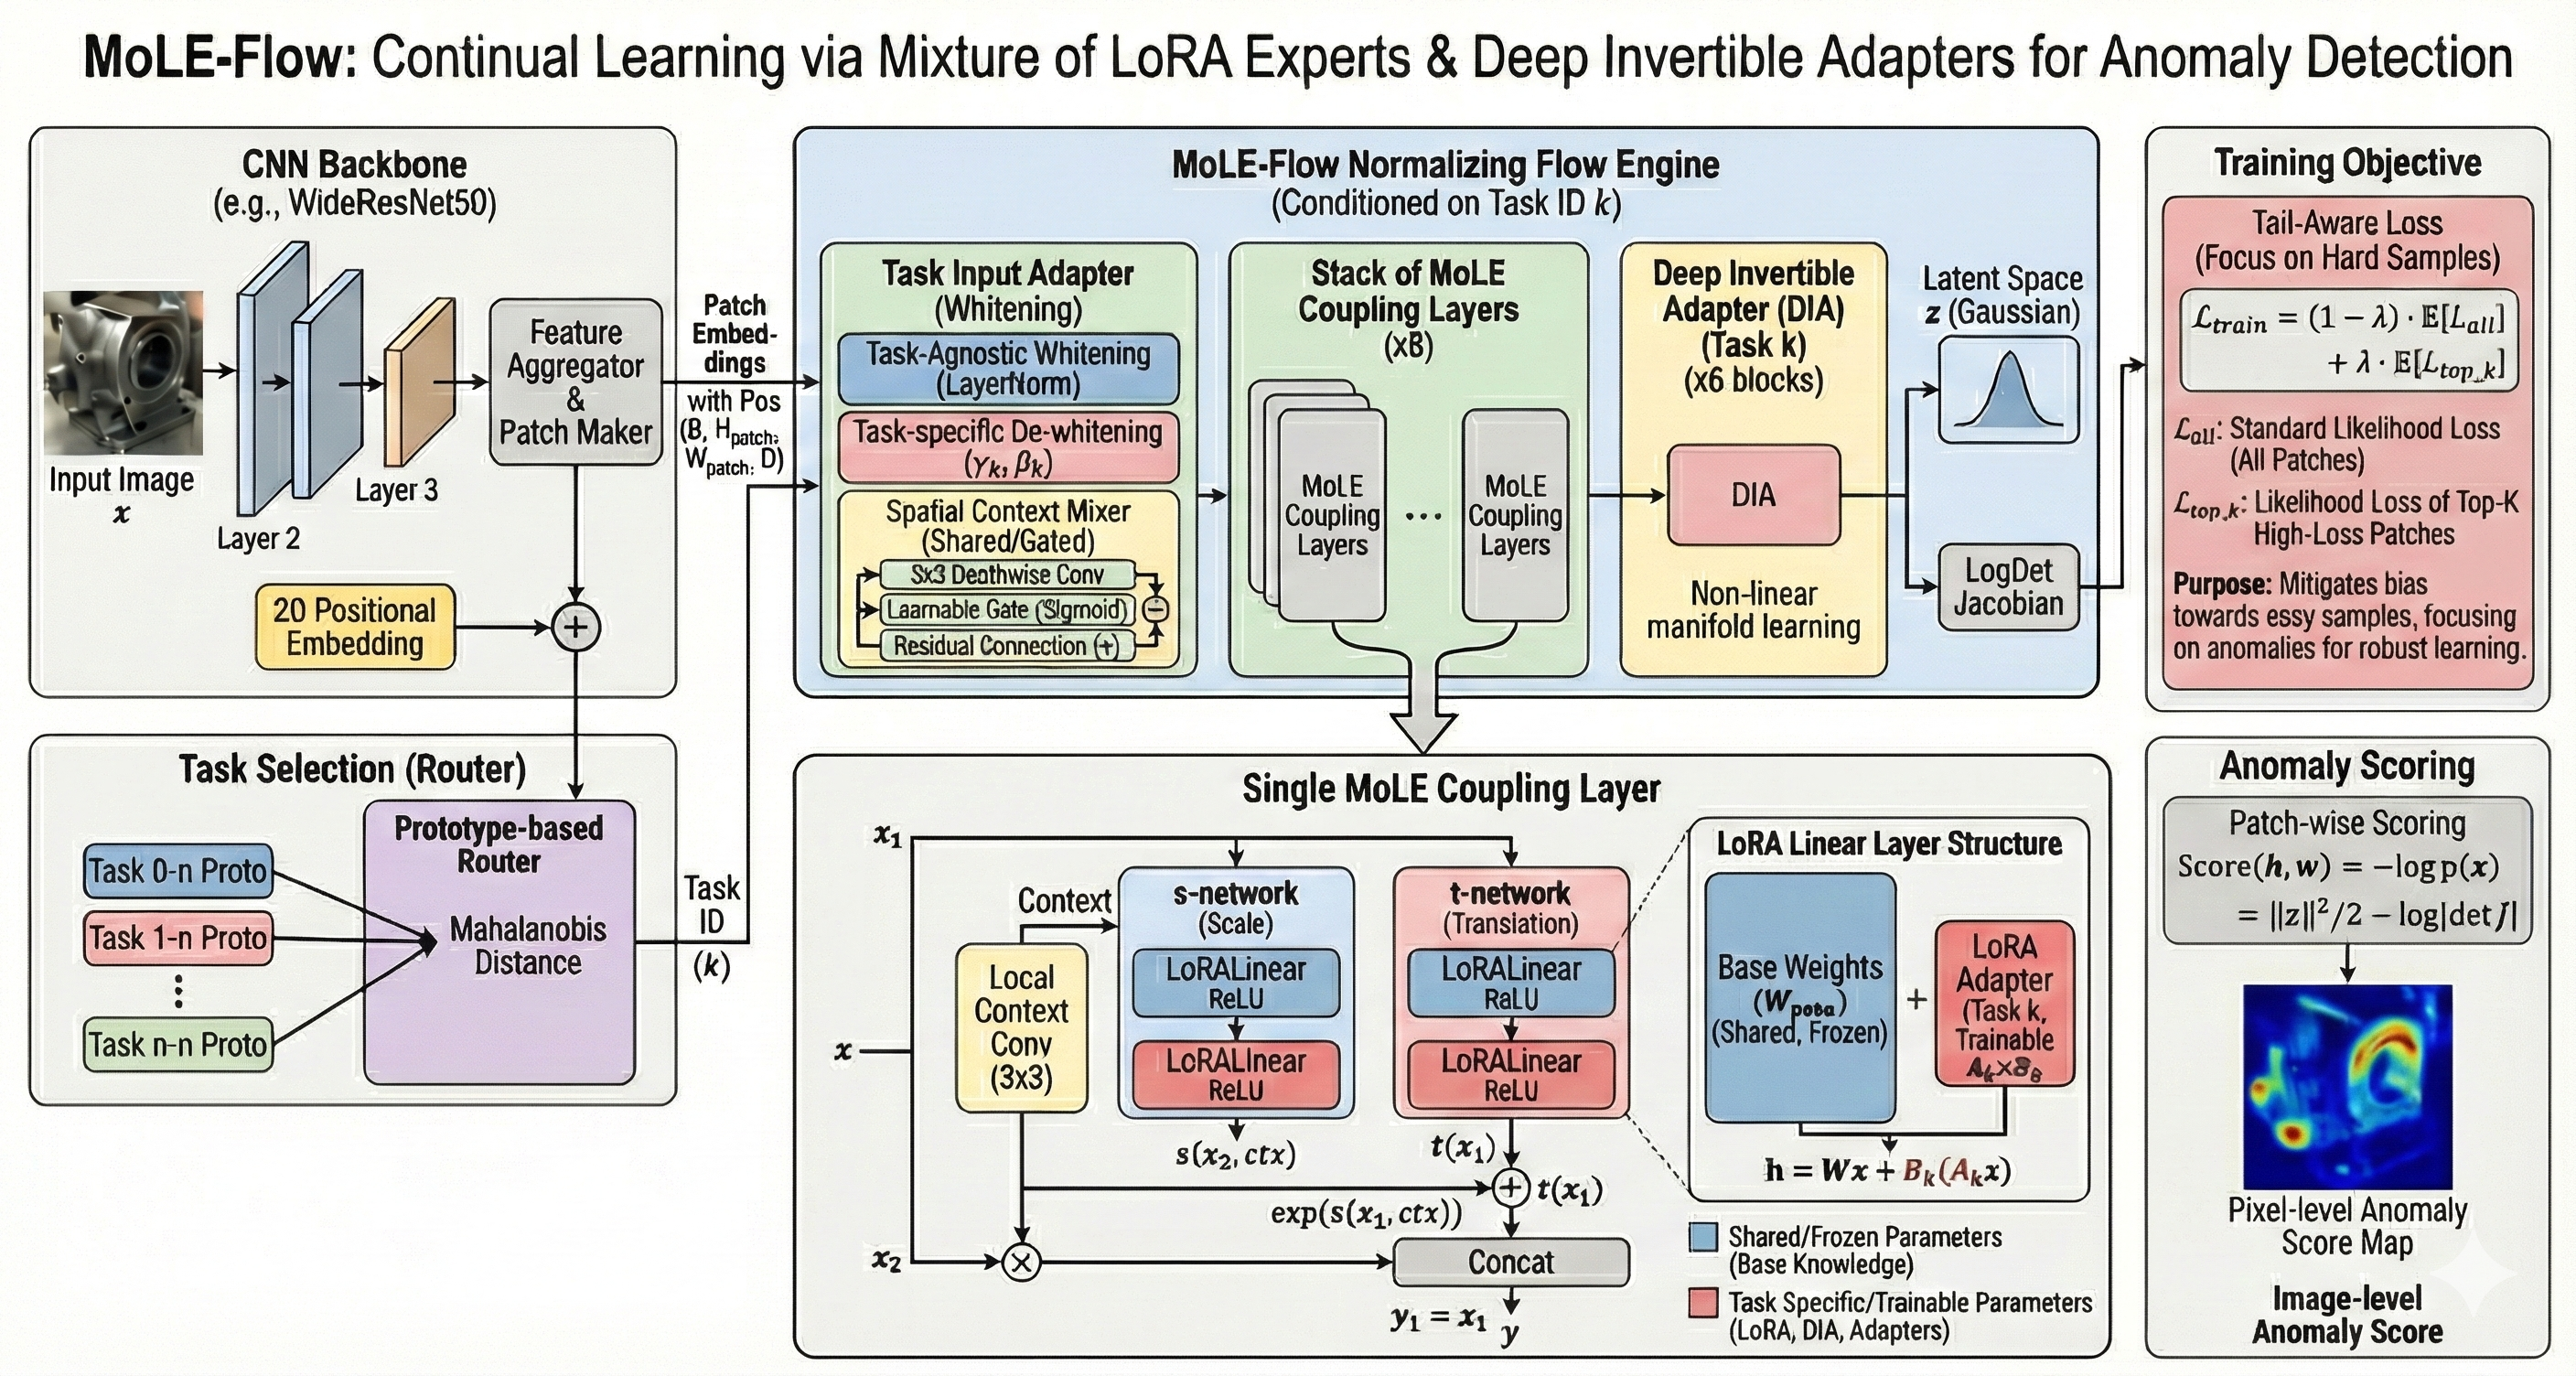
\includegraphics[width=\textwidth]{figures/main2.png}
    \caption{Overview of the proposed \textbf{MoLE-Flow} framework for continual anomaly detection on industrial images. Given sequential tasks, the base normalizing flow backbone is learned on the first task and then frozen. For each new task, only lightweight task-specific adapters (WhiteningAdapter, LoRA, DIA) are trained. At inference time, the prototype-based Mahalanobis router assigns each sample to the most relevant expert without requiring task ID.}
    \label{fig:main_figure}
\end{figure}

본 섹션에서는 Continual learning scenario 환경에서 anomaly detection을 수행하기 위한 방법인 MoLE-Flow(Mixture of LoRA Experts with Normalizing Flow for Continual Anomaly Detection) 프레임워크를 제안한다.
MoLE-Flow는 크게 특징 추출기, MoLE 기반 Normalizing Flow, 작업별 어댑터, 그리고 프로토타입 라우터로 구성되며, 다음 다섯 가지 핵심 기여를 제안한다:
\begin{enumerate}
\item \textbf{MoLE (Mixture of LoRA Experts)}: Normalizing Flow의 coupling 블록에 LoRA를 적용하여 작업별 경량 적응을 가능하게 하는 MoLESubnet 구조
\item \textbf{WhiteningAdapter}: 작업 간 특징 분포 차이를 정렬하기 위한 whitening 후 제약된 de-whitening 기반 적응 모듈
\item \textbf{Deep Invertible Adapter (DIA)}: 선형 LoRA의 한계를 극복하는 비선형 가역 적응 모듈
\end{enumerate}

\subsection{Overall Architecture}
\label{sec:overview}

MoLE-Flow는 사전 학습된 Backbone을 통해 이미지의 패치 임베딩을 추출한 후, Normalizing Flow를 통해 잠재 공간의 가우시안 분포로 매핑하는 구조를 가진다.
지속 학습 환경에 대응하기 위한 핵심 전략은 \textbf{Parameter Isolation}으로, Backbone과 Base NF의 파라미터는 공유하거나 고정하면서, 작업 특화 특징은 LoRA(Low-Rank Adaptation)와 DIA(Deep Invertible Adapter)에만 저장함으로써 메모리 효율성과 작업 간 간섭 방지를 동시에 달성한다.
전체 파이프라인은 다음과 같다:
\begin{enumerate}
\item Backbone으로부터 특징 추출 및 패치 임베딩 생성
\item Positional Encoding 생성 후 패치 임베딩에 추가
\item Task Adapters (Whitening)를 통한 작업 특화 특징 보존
\item Spatial Context Mixer를 통한 주변 문맥 정보 혼합
\item Normalizing Flow를 통한 확률 분포 추정
\item Likelihood 계산
\end{enumerate}

수식으로 표현하면:
\begin{equation}
\label{eq:pipeline}
\mathbf{x} \xrightarrow{\text{Backbone}} \mathbf{F} \xrightarrow{\text{PE}} \mathbf{F}' \xrightarrow{\text{Whitening}} \hat{\mathbf{F}} \xrightarrow{\text{SCM}} \tilde{\mathbf{F}} \xrightarrow{\text{NF+LoRA}} \mathbf{z}' \xrightarrow{\text{DIA}} (\mathbf{z}, \log|\det \mathbf{J}|)
\end{equation}

첫 번째 작업(Task 0)에서 Base와 작업 특화 Normalizing Flow 요소(LoRA, Whitening Adapter, DIA)를 모두 학습한 후, Base 파라미터는 동결된다.

\subsection{Feature Extraction \& Preprocessing}
\label{sec:feature_extraction}

입력 이미지의 특징을 추출하고 각 작업별 전문가를 학습시키기 위한 입력으로 사용하기 위해 다음과 같은 전처리를 수행한다.

\subsubsection{Feature Extractor \& Patch Embedding}
\begin{itemize}
    \item 사전 학습된 Feature Extractor를 통해 특징을 추출한다.
    \item 이때 intermediate layer의 출력을 활용하여 다중 스케일 정보(multi-scale information)를 얻는다.
    \item PatchCore와 유사하게 입력 이미지의 지역적 특성을 추출한다.
    \item 추출된 특징 맵을 패치 단위로 분할한 뒤 풀링 과정을 거쳐 패치 임베딩을 생성한다.
    \item 최종적으로 $\mathbf{F} \in \mathbb{R}^{B \times H \times W \times D}$ 형태의 패치 임베딩을 얻으며, 여기서 $H \times W$는 패치 그리드 크기, $D$는 특징 차원이다.
\end{itemize}

\subsubsection{Positional Encoding}
\begin{itemize}
    \item Normalizing Flow는 permutation invariance 특성을 갖기 때문에, 2차원 구조가 아닌 patch embedding 각각이 독립적으로 처리된다.
    \item 각 패치의 공간적 위치 정보를 보존하기 위해 2D sinusoidal positional encoding $\mathbf{P}$를 패치 임베딩에 더한다.
    \item 수식으로 표현하면 다음과 같다:
\begin{equation}
\mathbf{F}' = \mathbf{F} + \mathbf{P}, \quad \mathbf{P} \in \mathbb{R}^{H \times W \times D}
\end{equation}
\end{itemize}

%=========================================================================================================
\subsection{Whitening Adapter}
%=========================================================================================================

\label{sec:adapters}
\begin{itemize}
\item MoLE-Flow는 첫 번째 작업 학습 이후 Base Flow의 파라미터를 동결(Freeze)
\item 이는 모델이 초기 학습 데이터의 분포 통계량에 피팅됨을 의미
\item 새로운 작업의 입력 분포가 이와 크게 다를 경우(Covariate Shift), 다음과 같은 문제 발생:
    \begin{itemize}
    \item 고정된 Base Network의 가중치는 최적의 활성화를 일으키지 못함
    \item 제한된 용량(Low-Rank)을 가진 LoRA가 전역적인 분포 차이까지 보정해야 하는 과도한 부담
    \item 학습 초기 수렴 지연 및 최적화 난이도 증가
    \end{itemize}
\item Whitening Adapter 도입을 통해 이를 해결하고자 함:
    \begin{itemize}
    \item 입력 데이터를 강제로 표준 정규 분포로 정렬(Alignment)
    \item 고정된 Base Flow가 항상 일관된 스케일의 입력을 처리하도록 보장
    \item LoRA가 분포 보정이 아닌 작업 고유의 미세 특징 학습에만 집중 가능
    \item 파라미터 분리 구조 하에서 학습 효율성과 안정성 극대화
    \end{itemize}
\end{itemize}

\textbf{Whitening Adapter는 Whitening과 De-whitening의 두 단계로 구성됨.}

\subsubsection{\textbf{Task-Agnostic Whitening}} 
\begin{itemize}
\item 입력 특징 $\mathbf{F}'$에 대해 학습 파라미터가 없는 LayerNorm 적용
\item 평균 0, 분산 1의 표준 정규 분포로 변환:
\begin{equation}
\mathbf{x}_{\text{white}} = \text{LayerNorm}(\mathbf{F}', \text{elementwise\_affine}=\text{False}) = \frac{\mathbf{F}' - \mathbb{E}[\mathbf{F}']}{\sqrt{\text{Var}[\mathbf{F}'] + \epsilon}}
\end{equation}
\item Task 0 이후 Base Flow는 동결되므로, 새로운 작업의 입력 분포가 달라지면 모델이 제대로 반응하지 못함
\item 새로운 작업의 데이터가 들어와도 강제 정규화를 통해 입력을 표준화하여 분포의 스케일 차이를 미리 제거
\item Normalizing Flow의 최적화 난이도를 낮추고 학습 안정성 확보
\item 모든 데이터를 표준 정규 분포로 정규화한 후, De-whitening을 통해 Base Flow의 최적 동작 범위 내로 재조정
\end{itemize}

\subsubsection{\textbf{Task-Specific De-whitening}} 
\begin{itemize}
\item Whitening으로 제거된 통계적 특성에 \textbf{해당 작업을 가장 잘 표현할 수 있는 최적의 통계적 특성을 다시 부여}
\item 단순 복원이 아닌, \textbf{고정된 Base Flow가 처리하기 가장 효율적인 형태로 데이터를 재조정(Recalibration)}
\item 정규화된 특징 $\mathbf{x}_{\text{white}}$에 대해 작업별 학습 가능한 파라미터 $\gamma_t$(스케일)와 $\beta_t$(이동)를 적용한 아핀 변환:
\begin{align}
\gamma_t &= 0.5 + 1.5 \cdot \sigma(\gamma_{\text{raw}}) \\
\beta_t &= 2.0 \cdot \tanh(\beta_{\text{raw}}) \\
\hat{\mathbf{F}}_t &= \gamma_t \odot \mathbf{x}_{\text{white}} + \beta_t
\end{align}
여기서 $\sigma(\cdot)$는 시그모이드 함수

\item De-whitening 단계에서 작업별 학습 파라미터를 통해 각 작업의 고유한 특성을 복원
\item 단순한 원래 분포의 복원이 아니라, \textbf{고정된 모델의 매니폴드(Manifold) 상에서 각 작업 데이터가 가장 잘 표현될 수 있도록 최적의 통계적 위치를 학습하는 과정}
\item 모든 작업에서 모든 특징 채널이 동등하게 중요한 것은 아니므로, $\gamma_t$는 채널별로 특징의 중요도를 조절:
    \begin{itemize}
    \item $\gamma_t$ 값 증가 $\rightarrow$ 해당 특징 증폭, Flow 모델이 더 민감하게 반응
    \item $\gamma_t$ 값 감소 $\rightarrow$ 해당 특징 억제, 노이즈로 간주
    \item 예시: '가죽' 작업에서는 미세한 질감(Texture) 채널의 $\gamma_t$ 증가, '나사' 작업에서는 전체적인 형태(Shape) 채널의 $\gamma_t$ 증가
    \end{itemize}
\end{itemize}

\paragraph{아핀 변환을 사용하는 이유:}
De-whitening에서 아핀 변환(Affine Transformation, $\mathbf{y} = \gamma \odot \mathbf{x} + \beta$)을 사용하는 이유는 \textbf{통계적 특성(평균, 분산)만 정확하게 조절하고, 데이터가 가진 본질적인 구조(Shape/Pattern)는 훼손하지 않기 위해서}이다.

\begin{itemize}
\item \textbf{통계적 정합성 (Statistical Consistency):} 
    \begin{itemize}
    \item 정규 분포를 다른 정규 분포로 변환하는 가장 자연스러운 방법은 아핀 변환이다.
    \item Whitening은 데이터를 표준 정규 분포 $\mathcal{N}(0, 1)$로 만들고, De-whitening은 이를 작업별 고유 분포 $\mathcal{N}(\mu_t, \sigma_t^2)$로 이동시킨다.
    \item 비선형 변환(예: $x^2$, $\exp(x)$)을 사용하면 분포의 모양 자체가 왜곡되어 정규 분포의 성질(Bell curve)을 잃어버리며, 이는 가우시안 기반 Normalizing Flow의 처리를 어렵게 만든다.
    \end{itemize}

\item \textbf{구조 보존 (Structure Preservation):}
    \begin{itemize}
    \item 아핀 변환은 공간을 늘리거나(Scale), 이동(Shift)만 하므로 \textbf{직선은 직선으로 남고, 평행선은 평행하게 유지}된다.
    \item 이미지 패치 내부의 픽셀 관계는 물체의 형상을 나타내므로, 아핀 변환은 이미지가 조금 밝아지거나 대비가 강해질 뿐 "고양이"가 "강아지"처럼 보이게 모양이 바뀌지 않는다.
    \item 반면 비선형 변환은 공간을 구부리거나 비틀어 직선이 곡선이 되고 모양이 뒤틀리므로, \textbf{데이터의 내용(Content) 자체를 변질}시킬 위험이 있다.
    \item Adapter의 역할은 "입력의 톤(Tone)을 맞추는 것"이지, "내용을 재창조하는 것"이 아니므로 형태를 보존하는 아핀 변환이 최적이다.
    \end{itemize}

\item \textbf{역할 분담 (Division of Labor):}
    \begin{itemize}
    \item MoLE-Flow 전체 구조에서 Adapter는 서로 다른 도메인(가죽, 나사)의 \textbf{시작점(Start Point)을 맞춰주는 역할}로, 가장 기초적인 1차 모멘트(평균)와 2차 모멘트(분산)만 빠르고 정확하게 맞추면 된다.
    \item 실제 데이터의 복잡하고 비선형적인 분포 모델링은 Base Flow와 LoRA가 담당한다.
    \item Adapter가 굳이 복잡한 비선형 변환을 수행하여 연산량을 늘리고 최적화를 어렵게 만들 필요가 없으며, 이는 Batch Normalization이 학습 가능한 파라미터 $\gamma$, $\beta$를 두어 표현력을 복원하는 원리와 동일하다.
    \end{itemize}
\end{itemize}

결론적으로, Affine trnasformation은 \textbf{데이터의 본질은 건드리지 않으면서, 모델이 편식하지 않게 통계적 특성만 맞춰주는 가장 안전하고 효율적인 방법}이다.

\noindent 결과적으로 Whitening Adapter는:
\begin{itemize}
\item Whitening을 통해 불필요한 분포 격차를 제거
\item De-whitening을 통해 필요한 작업 고유의 특성을 학습된 형태로 복원
\item 입력 데이터의 글로벌한 표준화와 작업별 최적화를 동시에 달성
\item Base Flow는 Task 0의 데이터 분포에 최적화되어 고정되어 있으므로, 새로운 작업의 데이터가 "Task 0의 매니폴드 영역"과 동떨어져 있으면 Base Flow의 활성 함수들이 제대로 작동하지 않음
\item De-whitening은 $\gamma_t$와 $\beta_t$를 조절하여 정규화된 데이터를 Base Flow가 학습했던 익숙한 영역 근처로 매핑하고, 새로운 데이터가 Base Flow의 활성 함수들이 가장 잘 작동하는 구간(Active Region)에 위치하도록 보장
\item 고정된 Base Flow의 효과적인 재활용을 가능하게 하며, 지속 학습 환경에서 안정적이고 효율적인 학습을 보장
\end{itemize}

%=========================================================================================================
\subsection{\textbf{Spatial Context Mixer}}
%=========================================================================================================
\label{sec:spatial_mixer}

\subsubsection{\textbf{Motivation: Addressing the I.I.D. Assumption}}
\begin{itemize}
    \item Normalizing Flow 기반 모델은 계산의 효율성을 위해 이미지의 전체 우도(Likelihood)를 개별 패치 우도의 곱으로 근사한다.
\end{itemize}
\begin{equation}
    p(\mathbf{X}) \approx \prod_{u=1}^{H} \prod_{v=1}^{W} p(\mathbf{x}_{u,v})
\end{equation}
\begin{itemize}
    \item 이 식은 위치 $(u, v)$의 특징 벡터 $\mathbf{x}_{u,v}$가 인접한 이웃들과 독립적(Independent and Identically Distributed, i.i.d.)이라고 가정한다.
    \item 이러한 가정은 \textbf{구조적 사각지대(Structural Blind Spot)}를 야기한다.
\end{itemize}
\begin{itemize}
    \item \textbf{공간적 상관관계의 누락:} 긁힘(Scratch)이나 얼룩(Stain)과 같은 미세 결함은 단일 패치 내부의 값보다는 주변 패치와의 \textbf{불연속성(Discontinuity)}으로 정의된다. 그러나 Base Flow는 패치를 독립적으로 처리하므로 이러한 국소적 대조(Local Contrast)를 인지하지 못한다.
    \item \textbf{문맥 정보의 부재:} 정상 데이터의 분포는 주변 문맥에 따라 달라질 수 있다. 독립적인 처리는 $p(\mathbf{x}_{u,v} | \text{Neighbors})$와 같은 조건부 확률을 모델링할 수 없다.
\end{itemize}

\subsubsection{\textbf{Mechanism: Gated Depthwise Aggregation}}
\begin{itemize}
    \item 이러한 한계를 극복하기 위해 우리는 Base Flow 입력 직전에 \textbf{Spatial Context Mixer}를 도입하였다.
    \item 이 모듈은 파라미터 효율성을 극대화하면서, 각 패치가 주변 정보를 물리적으로 집계할 수 있도록 설계되었다.
\end{itemize}

\begin{itemize}
    \item \textbf{Spatial Aggregation (Depthwise Convolution):} 
    \begin{itemize}
        \item Mixer는 채널 간의 간섭 없이 오직 공간적 정보만을 통합하기 위해 \textbf{Depthwise Convolution}을 사용한다.
    \end{itemize}
    \begin{equation}
        \mathbf{C}^{(k)}_{u,v} = \sum_{i=-1}^{1} \sum_{j=-1}^{1} \mathbf{W}^{(k)}_{i,j} \cdot \mathbf{x}^{(k)}_{u+i, v+j}
    \end{equation}
    여기서 $\mathbf{x}^{(k)}$는 $k$번째 채널의 입력 특징 맵, $\mathbf{W}^{(k)}$는 해당 채널의 $3 \times 3$ 커널 가중치, $\mathbf{C}$는 추출된 문맥 특징(Context Feature)이다. 이를 통해 각 특징 벡터는 자신의 위치뿐만 아니라 8-방향 이웃의 텍스처 정보를 집계한다.

    \begin{itemize}
        \item \textbf{Adaptive Interpolation (Learnable Gating):} 단순한 잔차 연결(Residual Addition) 대신, 모델은 원본 정보와 문맥 정보의 반영 비율을 스스로 결정하는 \textbf{적응형 보간(Adaptive Interpolation)} 메커니즘을 사용한다.
        \begin{equation}
            \alpha = \sigma(\theta_{\text{gate}})
        \end{equation}
        \begin{equation}
            \mathbf{z}_{u,v} = (1 - \alpha) \cdot \mathbf{x}_{u,v} + \alpha \cdot \mathbf{C}_{u,v}
        \end{equation}
        여기서 $\sigma(\cdot)$는 시그모이드(Sigmoid) 함수이며, $\theta_{\text{gate}}$는 학습 가능한 스칼라 파라미터이다.

        \item \textbf{Design Rationale:} 이러한 게이팅 구조는 학습 초기($\alpha \approx 0.5$ 또는 초기화에 따라 조절)에 원본 특징과 문맥 특징을 균형 있게 학습하다가, 최적화 과정에서 태스크에 따라 공간 정보의 중요도($\alpha$)를 동적으로 조절할 수 있게 한다. 예를 들어, 텍스처가 균일한 표면(가죽 등)에서는 $\alpha$를 높여 주변 정보를 적극 활용하고, 복잡한 객체에서는 조절하는 식이다.
    \end{itemize}
\end{itemize}

\subsubsection{\textbf{Effect: Pseudo-Dependency Modeling}}
최종적으로 생성된 특징 벡터 $\mathbf{z}_{u,v}$는 수학적으로는 Base Flow에 독립적인 개체로 입력되지만, 정보적으로는 이미 주변 이웃의 상태 $\mathcal{N}_{u,v}$를 내포하고 있다.
\begin{equation}
    \mathbf{z}_{u,v} \approx \text{Encode}(\mathbf{x}_{u,v} \oplus \mathcal{N}_{u,v})
\end{equation}
결과적으로 Base Flow는 구조 변경 없이도 $\mathbf{z}_{u,v}$를 통해 간접적으로 조건부 확률 $p(\mathbf{x}_{u,v} | \mathcal{N}_{u,v})$을 학습하는 효과(Pseudo-Dependency)를 얻게 되며, 이는 구조적 이상 탐지 성능을 비약적으로 향상시킨다.

%=========================================================================================================
\subsection{MoLE-Flow}
%=========================================================================================================
\label{sec:moleflow}

Normalizing Flow는 Feature Extractor를 통해 생성된 입력 이미지들의 패치 임베딩을 가우시안으로 매핑하며 분포를 학습하고 추정하기 위한 도구로 사용된다.
기본적으로 RealNVP 기반의 구조를 사용하며, 각 coupling 블록에 LoRA 어댑터를 적용하여 작업별 경량 적응을 가능하게 하는 핵심 구조이다.
MoLE-Flow의 전체 구조는 다음과 같이 구성된다:
\begin{itemize}
\item Spatial Context Mixer
\item MoLEContextSubnet: 분포 학습
\item Deep Invertible Adapter (DIA): 비선형 매니폴드 학습
\end{itemize}

\subsubsection{MoLEContextSubnet}

MoLEContextSubnet들이 직렬로 연결된 구조를 가진다.
각 블록은 입력 데이터를 분할하여 가역 변환을 수행하며, 다음과 같은 구조로 설계되어 있다.

\paragraph{Spatial Structure Recovery:}
Normalizing Flow는 기본적으로 패치 임베딩들을 평탄화(flatten)하여 패치들을 독립적으로 처리한다.
문맥 정보를 추출하기 위해 일시적으로 공간 구조를 복원한다.

\paragraph{Context Extraction \& Adaptive Gating:}
복원된 공간 특징 $\hat{\mathbf{x}}$에 대해 $3 \times 3$ Depthwise Convolution을 적용하여 지역적 문맥 $\mathbf{c}(\hat{\mathbf{x}})$를 추출한다.
이후, 학습 가능한 파라미터 $\theta_{\text{scale}}$을 통해 문맥 정보의 반영 비율 $\alpha$를 동적으로 조절한다:
\begin{equation}
\alpha = \alpha_{\max} \cdot \sigma(\theta_{\text{scale}})
\end{equation}

\noindent 여기서 $\sigma$는 시그모이드 함수이며, $\alpha_{\max}$는 문맥 정보의 최대 영향력을 제한하는 상수이다.
계산된 문맥 특징은 다시 평탄화되어 입력 $\mathbf{x}$와 동일한 차원을 갖는다.
이 문맥 특징은 조건(condition)으로 활용되어 $\mathbf{x}$를 변환할 때 스케일($\mathbf{s}$)과 이동($\mathbf{t}$) 값을 계산하는 데 힌트로 사용된다.

\paragraph{Channel Splitting:}
입력 벡터 $\mathbf{x}$를 채널 축을 기준으로 두 개의 부분 $\mathbf{x}_1$, $\mathbf{x}_2$로 분할한다.

\paragraph{LoRA-based Coupling Layer:}
LoRALinear 층은 MoLE-Flow에서 파멸적 망각을 막고, 새로운 작업을 효율적으로 학습하기 위해 \textbf{고정된 지식(Base)}과 \textbf{적응형 지식(LoRA)}을 병렬로 처리하는 구조를 가진다:
\begin{equation}
\mathbf{h}(\mathbf{x}) = \mathbf{W}_{\text{base}}\mathbf{x} + \frac{\alpha}{r}(\mathbf{B}\mathbf{A})\mathbf{x} + (\mathbf{b}_{\text{base}} + \mathbf{b}_t)
\end{equation}

\begin{itemize}
\item \textbf{Base Linear (Frozen Anchor)}: Task 0에서 학습된 후 고정되며, 모든 작업이 공유하는 범용적인 특징 변환 역할을 수행한다. 이미지 패치 분포의 가장 기초적인 통계적 특성을 추출하고 변환하는 뼈대 역할을 수행한다.
\item \textbf{LoRA Linear (Task-Specialist)}: 고정된 Base Linear가 처리하지 못하는 작업 고유의 분포 특성을 보정한다. Base가 대략적인 방향을 잡으면, LoRA는 그 방향을 작업에 맞게 미세 조정하는 역할을 수행한다. 각 작업마다 새로운 $\mathbf{A}$, $\mathbf{B}$ 행렬 세트가 생성되며, 해당 작업 학습 시에만 업데이트된다.
\end{itemize}

\paragraph{Context-Aware s-network (Scale Prediction):}
스케일 파라미터 $\mathbf{s}$를 예측하는 네트워크는 원본 특징 $\mathbf{x}$와 게이팅된 문맥 $\mathbf{ctx}$를 결합(concat)하여 입력으로 사용한다.
스케일 변화가 주변 패치와의 상호작용에 민감하다는 점을 반영한 설계이다:
\begin{equation}
\mathbf{s} = \text{Layer2}_s(\text{ReLU}(\text{Layer1}_s([\mathbf{x}; \mathbf{ctx}])))
\end{equation}

\paragraph{Context-Free t-network (Translation Prediction):}
이동 파라미터 $\mathbf{t}$를 예측하는 네트워크는 문맥 정보 없이 오직 원본 특징 $\mathbf{x}$만을 입력으로 사용한다.
이는 데이터 분포의 중심(shift)이 주변 정보보다는 패치 고유의 특성에 종속된다는 inductive bias를 반영한 것이다:
\begin{equation}
\mathbf{t} = \text{Layer2}_t(\text{ReLU}(\text{Layer1}_t(\mathbf{x})))
\end{equation}

\noindent 최종적으로 두 네트워크의 출력 $\mathbf{s}$와 $\mathbf{t}$는 Coupling Layer의 변환 수식에 활용된다.

\subsubsection{Deep Invertible Adapter (DIA)}

DIA는 Normalizing Flow 출력단에 위치하며, MoLESubnet이 처리하지 못한 작업 특화 비선형 매니폴드를 정밀 보정한다.
Affine Coupling Block으로 구성되며, 각 작업별로 독립적인 파라미터가 분리되어 있다.

수학적으로, 전체 변환과 밀도 추정은 다음과 같이 표현된다:
\begin{equation}
\mathbf{z}_{\text{final}} = f_{\text{DIA}}^{(t)}(\mathbf{z}_{\text{base}}), \quad \log p(\mathbf{x}) = \log p(\mathbf{z}_{\text{final}}) + \log|\det \mathbf{J}_{\text{base}}| + \log|\det \mathbf{J}_{\text{DIA}}|
\end{equation}

각 AffineCouplingBlock의 변환:
\begin{align}
[\mathbf{x}_1, \mathbf{x}_2] &= \text{Split}(\mathbf{x}) \\
\mathbf{s}, \mathbf{t} &= \text{SimpleSubnet}(\mathbf{x}_1) \\
\mathbf{y}_2 &= \mathbf{x}_2 \odot \exp(\alpha_{\text{clamp}} \cdot \tanh(\mathbf{s}/\alpha_{\text{clamp}})) + \mathbf{t} \\
\mathbf{y} &= \text{Concat}(\mathbf{x}_1, \mathbf{y}_2)
\end{align}

DIA의 핵심 장점:
\begin{enumerate}
\item \textbf{비선형 매니폴드 적응}: 선형 LoRA가 표현할 수 없는 복잡한 분포 변환을 학습한다.
\item \textbf{가역성 보장}: 정규화 흐름의 밀도 추정 속성이 유지되므로, 이상 점수의 확률적 해석이 보존된다.
\item \textbf{완전한 작업 분리}: 작업별로 완전히 독립적인 파라미터를 사용하여 작업 간 간섭이 없다.
\item \textbf{후처리 위치}: 기반 NF의 뒷단에 위치하여, 기반 NF가 학습한 범용 변환을 먼저 적용하고 DIA가 작업 특화 조정을 수행한다.
\end{enumerate}

\subsection{Training Objective}
\label{sec:training_objective}

모델의 학습과 이상 탐지는 입력 데이터가 잠재 공간의 정규 분포로 얼마나 잘 매핑되는지를 측정하는 Log-likelihood 계산을 통해 이루어진다.
이 과정은 크게 Forward 변환 및 Jacobian 누적, 잠재 확률 계산, 그리고 최종 likelihood 산출을 통해 이루어진다.

\subsubsection{Likelihood Calculation}

사전 학습된 특징 추출기로부터 생성된 입력 패치 임베딩은 잠재 변수 $\mathbf{z}$로 변환되며, 각 변환 단계의 부피 변화율인 log-determinant of Jacobian이 누적된다.

\paragraph{Transformation Flow:}
입력 $\mathbf{x}$는 Task Adapter, Spatial Mixer, MoLESubnet, DIA를 순차적으로 통과하며 최종 잠재 벡터 $\mathbf{z}$로 변환된다.

\paragraph{Jacobian Accumulation:}
Flow와 DIA를 거치는 동안 발생된 log determinant Jacobian 값들이 합산된다:
\begin{equation}
\log|\det \mathbf{J}_{\text{total}}| = \log|\det \mathbf{J}_{\text{flow}}| + \log|\det \mathbf{J}_{\text{DIA}}|
\end{equation}

\paragraph{Latent Probability:}
최종 잠재 벡터 $\mathbf{z}_{\text{final}}$이 표준 정규분포를 따른다고 가정하고, 각 패치 위치에서의 log probability density를 계산한다:
\begin{equation}
\log p(\mathbf{z}_{\text{final}}) = -\frac{1}{2}\|\mathbf{z}_{\text{final}}\|_2^2 - \frac{D}{2}\log(2\pi)
\end{equation}

\paragraph{Final Likelihood:}
변수 변환 공식에 따라 입력 공간에서의 log likelihood는 다음과 같이 계산된다:
\begin{equation}
\log p(\mathbf{x}) = \log p(\mathbf{z}_{\text{final}}) + \log|\det \mathbf{J}_{\text{total}}|
\end{equation}

\subsubsection{Tail-Aware Loss}

일반적인 NF의 학습 방식을 따르는 경우 이미지 내 모든 패치의 우도 평균을 최대화하게 된다.
그러나 이는 모델이 대다수의 학습하기 ``쉬운'' 정상 패치에만 집중하게 되고, 분포의 꼬리(Tail)에 위치한 ``어려운'' 패치나 이상 징후를 간과하게 만드는 원인이 된다.

따라서 본 모델은 학습 시 Tail-Aware Loss를 도입하여, 전체 평균뿐만 아니라 손실 값이 높은 상위 $K\%$ 패치에 가중치를 두어 학습하도록 한다:
\begin{equation}
\mathcal{L}_{\text{train}} = (1 - \lambda) \cdot \mathbb{E}[\mathcal{L}_{\text{all}}] + \lambda \cdot \mathbb{E}[\mathcal{L}_{\text{top-k}}]
\end{equation}

\noindent 여기서 $\lambda = 0.3$, $\mathcal{L}_{\text{top-k}}$는 상위 5\% 고손실 패치의 평균 NLL이다.
이는 모델이 정상 분포의 경계(Boundary)를 더 명확하게 학습하도록 유도한다.

\subsection{Anomaly Scoring \& Inference}
\label{sec:inference}

본 모델의 추론 과정은 입력 이미지에서 특징을 추출하고, 이를 학습된 정상 분포와 비교하여 국소적인 이상 징후를 탐지한 뒤, 이를 하나의 신뢰할 수 있는 이미지 레벨 점수로 변환하는 일련의 파이프라인으로 구성된다.

\subsubsection{Step 1: Feature Extraction \& Embedding}

입력 이미지 $\mathbf{x}_{\text{img}} \in \mathbb{R}^{H \times W \times C}$가 모델에 입력되면, 다음과 같은 전처리를 거친다:
\begin{enumerate}
\item \textbf{Backbone}: 사전 학습된 ViT를 통과하여 다중 스케일 특징 맵을 추출한다.
\item \textbf{Patchify}: 특징 맵을 패치 단위로 분할하고 풀링하여 $N$개의 패치 임베딩 벡터를 생성한다.
\item \textbf{Positional Encoding}: 각 패치의 위치 정보 $(h, w)$에 해당하는 Positional Embedding을 더하여 최종 입력 벡터 $\mathbf{x}$를 완성한다.
\end{enumerate}

\noindent 출력: $\mathbf{x} \in \mathbb{R}^{B \times H_{\text{patch}} \times W_{\text{patch}} \times D}$

\subsubsection{Step 2: Task Routing \& Adapter Activation}

작업 ID가 주어지지 않았다면, 라우터가 작동한다:
\begin{enumerate}
\item \textbf{Prototype Matching}: 입력 특징의 평균과 저장된 작업별 프로토타입 간의 Mahalanobis 거리를 계산한다:
\begin{equation}
t^* = \argmin_t D_M(\mathbf{f}, t), \quad D_M(\mathbf{f}, t) = \sqrt{(\mathbf{f} - \boldsymbol{\mu}_t)^\top \boldsymbol{\Sigma}_t^{-1} (\mathbf{f} - \boldsymbol{\mu}_t)}
\end{equation}
\item \textbf{Selection}: 가장 거리가 가까운 작업 $t^*$를 선정하고, 해당 작업에 특화된 LoRA, Whitening, DIA 파라미터를 활성화한다.
\end{enumerate}

\noindent 기존의 연구들은 Task routing을 위해 별도의 inference 과정을 거친 뒤 얻은 작업 정보를 가지고 한 번 더 inference를 수행하여 이상 탐지를 수행한다.
그러나 본 방법론에서는 별도의 과정 없이 one-stage로 routing과 이상 탐지를 수행할 수 있다는 이점이 있다.

\subsubsection{Step 3: Distribution Mapping via MoLE-Flow}

활성화된 어댑터들을 사용하여 입력 $\mathbf{x}$를 잠재 공간의 $\mathbf{z}$로 변환한다.
이 과정에서 정상 데이터의 분포(가우시안)로 매핑을 시도한다:
\begin{equation}
\mathbf{z}, \log|\det \mathbf{J}| = \text{MoLE-Flow}_{t^*}(\mathbf{x})
\end{equation}

입력은 Whitening $\rightarrow$ Spatial Context $\rightarrow$ Base Flow + LoRA $\rightarrow$ DIA를 순차적으로 통과한다.
변환의 역할:
\begin{itemize}
\item \textbf{정상 패치}: 학습된 변환에 의해 원점(0) 근처의 $\mathbf{z}$로 매핑되며, 변환 과정(Jacobian)이 자연스럽다.
\item \textbf{이상 패치}: 정상 분포를 따르지 않으므로, $\mathbf{z}$가 원점에서 멀어지거나 변환 과정에서 부피가 비정상적으로 왜곡된다.
\end{itemize}

\subsubsection{Step 4: Patch-wise Anomaly Scoring}

각 패치 위치 $(h, w)$마다 ``이 패치가 얼마나 비정상적인가?''를 나타내는 점수를 계산한다.
이는 음의 로그 우도(Negative Log-Likelihood)로 정의된다:
\begin{equation}
\text{Score}_{(h,w)} = -\log p(\mathbf{x}_{(h,w)}) = \underbrace{\frac{1}{2}\|\mathbf{z}_{(h,w)}\|^2}_{\text{Distance Score}} \underbrace{- \log|\det \mathbf{J}|_{(h,w)}}_{\text{Distortion Score}}
\end{equation}

\noindent 결과물: 입력 이미지와 공간적으로 대응되는 \textbf{Anomaly Heatmap} (Shape: $H_{\text{patch}} \times W_{\text{patch}}$)이 생성된다.

\subsubsection{Step 5: Top-K Mean Aggregation}

생성된 히트맵을 하나의 이미지 레벨 이상 점수(Image-Level Anomaly Score)로 변환한다.
단순 평균이나 최대값이 아닌 \textbf{Top-K Mean} 방식을 사용하여 노이즈에 강건한 판단을 내린다.

\paragraph{Flatten \& Sort:}
$H \times W$ 크기의 히트맵을 1차원 벡터로 평탄화한 뒤, 점수가 높은 순서대로(내림차순) 정렬한다:
\begin{equation}
\mathbf{S}_{\text{sorted}} = \text{SortDesc}(\{\text{Score}_{(h,w)} \mid \forall h, w\})
\end{equation}

\paragraph{Top-K Selection:}
가장 이상도가 높은 상위 $K$개의 패치만 선택한다:
\begin{equation}
\mathbf{S}_{\text{top}} = \{S_{\text{sorted}}^{(1)}, S_{\text{sorted}}^{(2)}, \dots, S_{\text{sorted}}^{(K)}\}
\end{equation}

Top-K를 사용하는 이유:
\begin{itemize}
\item \textbf{vs Max}: 단일 픽셀 튐(Sensor Noise)에 의한 오탐(False Positive)을 방지한다.
\item \textbf{vs Mean}: 정상 영역이 압도적으로 많은 경우, 이상 신호가 희석(Dilution)되는 것을 막는다. 실제 결함은 보통 군집(Cluster)을 이루므로 $K$개의 강한 신호를 보는 것이 유리하다.
\end{itemize}

\paragraph{Averaging:}
선택된 $K$개 점수의 평균을 최종 이미지 점수로 확정한다:
\begin{equation}
\text{Final Image Score} = \frac{1}{K} \sum_{i=1}^{K} S_{\text{top}}^{(i)}
\end{equation}

\noindent 이 추론 과정은 ``패치 단위로 세밀하게 검사(Flow)''한 뒤, ``가장 의심스러운 부분들만 모아서 종합 판단(Top-K Aggregation)''하는 전략을 취한다.
이를 통해 미세한 스크래치(Screw)부터 구조적 결함(Transistor)까지 다양한 유형의 불량을 노이즈 간섭 없이 효과적으로 탐지할 수 있다.

\section{Experiments}
\label{sec:experiments}

본 섹션에서는 MoLE-Flow의 성능을 검증하기 위한 실험 설계를 제시한다.
실험은 크게 (1) 기존 방법론과의 비교를 통한 우수성 검증, (2) 각 모듈의 유효성을 확인하는 Ablation Study, (3) 지속 학습 특성 분석, (4) 정성적 결과 분석으로 구성된다.

\subsection{Experimental Setup}
\label{sec:exp_setup}

\subsubsection{Datasets}
산업 이상 탐지 분야의 대표적인 벤치마크 데이터셋들을 사용한다:

\begin{itemize}
\item \textbf{MVTec AD}~\cite{bergmann2019mvtec}: 15개의 산업 제품 클래스(bottle, cable, capsule, carpet, grid, hazelnut, leather, metal\_nut, pill, screw, tile, toothbrush, transistor, wood, zipper)를 포함하며, 총 5,354개의 고해상도 이미지로 구성된다. 주요 벤치마크로 사용한다.
\item \textbf{VisA}~\cite{zou2022spot}: 12개의 복잡한 산업 제품 클래스를 포함하며, MVTec AD보다 더 복잡한 텍스처와 미세한 결함을 포함한다. Cross-dataset 일반화 성능 평가에 사용한다.
\item \textbf{MPDD}~\cite{jezek2021deep}: 6개의 금속 부품 클래스를 포함하며, 금속 표면의 다양한 결함 유형을 제공한다.
\end{itemize}

\subsubsection{Evaluation Metrics}
이상 탐지 성능과 지속 학습 능력을 종합적으로 평가하기 위해 다음 지표들을 사용한다:

\paragraph{Detection Metrics:}
\begin{itemize}
\item \textbf{Image AUROC}: 이미지 수준 정상/이상 분류 성능. 본 연구의 주요 지표이다.
\item \textbf{Image AP}: 클래스 불균형 상황에서의 이미지 수준 성능.
\end{itemize}

\paragraph{Localization Metrics:}
\begin{itemize}
\item \textbf{Pixel AUROC}: 픽셀 수준 이상 영역 탐지 정확도.
\item \textbf{Pixel AP}: 클래스 불균형을 고려한 픽셀 수준 성능.
\item \textbf{PRO (Per-Region Overlap)}: 연결된 이상 영역별 IoU 기반 평가 지표. MVTec AD 벤치마크의 표준 메트릭으로, 다양한 크기의 결함에 대해 공정한 평가를 제공한다.
\end{itemize}

\paragraph{Continual Learning Metrics:}
\begin{itemize}
\item \textbf{Average Accuracy (ACC)}: 모든 작업에 대한 최종 평균 성능. $\text{ACC} = \frac{1}{T}\sum_{i=1}^{T}a_{T,i}$.
\item \textbf{Forgetting (F)}: 새로운 작업 학습 후 이전 작업 성능 하락 정도. $F = \frac{1}{T-1}\sum_{i=1}^{T-1}(a_{i,i} - a_{T,i})$. 낮을수록 좋다.
\item \textbf{Backward Transfer (BWT)}: 이전 작업에 대한 지식 전이 효과. $\text{BWT} = \frac{1}{T-1}\sum_{i=1}^{T-1}(a_{T,i} - a_{i,i})$. 0에 가까울수록 망각이 적다.
\item \textbf{Routing Accuracy}: Task ID 없이 올바른 전문가를 선택하는 정확도. MoLE-Flow의 핵심 기능이다. \textbf{Router Confusion이 성능 저하의 주요 원인이 될 수 있으므로} 이 지표를 별도로 상세 분석한다.
\end{itemize}

\subsubsection{Continual Learning Scenarios}
지속 학습 능력을 다각도로 검증하기 위해 다음 시나리오들을 설계한다:

\paragraph{Scenario A: Standard 5-Task Protocol}
MVTec AD의 15개 클래스를 5개 작업(각 3개 클래스)으로 구성한다:
\begin{itemize}
\item Task 0: leather, grid, transistor (텍스처 + 객체 혼합)
\item Task 1: carpet, zipper, hazelnut
\item Task 2: toothbrush, metal\_nut, screw
\item Task 3: wood, tile, capsule
\item Task 4: pill, cable, bottle
\end{itemize}
각 작업을 순차적으로 학습하며, 이전 데이터에는 접근하지 않는다 (No Replay).

\paragraph{Scenario B: Long Sequence (15-Task)}
15개 클래스를 각각 독립된 작업으로 구성하여 장기 지속 학습 시나리오를 평가한다. 이는 모델의 확장성(Scalability)과 장기 망각(Long-term Forgetting)을 검증한다.

\paragraph{Scenario C: Class Order Sensitivity}
동일한 클래스 집합에 대해 5개의 서로 다른 무작위 순서로 학습하여 순서 민감도를 분석한다.

\paragraph{Scenario D: Task 0 Dependency Analysis (Critical)}
MoLE-Flow는 Task 0에서 Base weights를 학습하고 이후 동결하는 구조이므로, \textbf{첫 번째 작업의 특성이 전체 성능에 영향을 미칠 수 있다}. 이를 검증하기 위해 다음 실험을 수행한다:
\begin{itemize}
\item \textbf{Texture-first}: 텍스처 클래스(carpet, leather, grid, wood, tile)를 Task 0으로 설정
\item \textbf{Object-first}: 객체 클래스(bottle, capsule, pill, toothbrush, transistor)를 Task 0으로 설정
\item \textbf{Mixed-first}: 텍스처와 객체를 혼합하여 Task 0으로 설정
\end{itemize}
이 실험을 통해 Task 0의 일반화 능력과 후속 작업에 대한 전이 학습 효과를 분석한다.

\subsubsection{Baseline Methods}
다음 범주의 방법론들과 비교한다:

\paragraph{Continual Anomaly Detection Methods:}
\begin{itemize}
\item \textbf{DNE}~\cite{li2022dne}: 분포 저장 기반의 최초 Continual AD 방법. 각 작업의 정상 분포 통계를 저장한다.
\item \textbf{UCAD}~\cite{lu2024ucad}: Prompt 기반 SOTA 방법. Vision Transformer의 prompt tuning을 활용한다.
\end{itemize}

\paragraph{Continual Learning + AD Adaptation:}
기존 지속 학습 방법을 이상 탐지에 적용한 baseline들:
\begin{itemize}
\item \textbf{EWC}~\cite{kirkpatrick2017ewc}: Elastic Weight Consolidation. 중요 파라미터에 정규화를 적용한다.
\item \textbf{LwF}~\cite{li2017lwf}: Learning without Forgetting. Knowledge Distillation 기반 방법.
\item \textbf{Replay-based}: 이전 작업 데이터의 일부를 저장하여 재학습에 활용한다.
\end{itemize}

\paragraph{Upper/Lower Bounds:}
\begin{itemize}
\item \textbf{Joint Training}: 모든 작업 데이터를 동시에 학습 (Upper Bound).
\item \textbf{Task-Separated}: 각 작업별 독립 모델 학습 (망각 없음, 메모리 비효율).
\item \textbf{Fine-tuning}: 단순 순차 학습 (Lower Bound, 심각한 망각).
\end{itemize}

\subsubsection{Implementation Details}

\paragraph{Network Configuration:}
\begin{itemize}
\item \textbf{Backbone}: ViT-Base-16 (ImageNet-21k pretrained), 동결
\item \textbf{Feature Aggregation}: 블록 $\{1, 3, 5, 11\}$에서 다중 스케일 특징 추출
\item \textbf{Normalizing Flow}: 8개의 Affine Coupling Layer, 클램핑 $\alpha = 1.9$
\item \textbf{LoRA}: rank = 64, scaling $\alpha$ = 1.0
\item \textbf{DIA}: 4개의 Affine Coupling Block
\end{itemize}

\paragraph{Training Configuration:}
\begin{itemize}
\item \textbf{Optimizer}: AdamW, weight decay = $1 \times 10^{-5}$
\item \textbf{Learning Rate}: $2 \times 10^{-4}$
\item \textbf{Batch Size}: 16
\item \textbf{Epochs}: 60 per task
\item \textbf{Input Size}: $224 \times 224$
\item \textbf{Tail-Aware Loss}: $\lambda = 0.5$, Top-K ratio = 5\%
\item \textbf{Log-det Regularization}: $\lambda_{\text{logdet}} = 10^{-4}$
\end{itemize}

모든 실험은 NVIDIA RTX 4090 GPU에서 PyTorch 2.0과 FrEIA 라이브러리를 사용하여 수행한다.

%==============================================================================
\subsection{Main Results}
\label{sec:main_results}

\subsubsection{Comparison with State-of-the-Art Methods}

표~\ref{tab:main_comparison}은 MVTec AD 데이터셋에서 5-Task 시나리오에 대한 주요 방법들과의 비교 결과를 보여준다.

\begin{table*}[t]
\centering
\caption{MVTec AD에서의 주요 방법론 비교 (5-Task Protocol). $\uparrow$: 높을수록 좋음, $\downarrow$: 낮을수록 좋음. 최고 성능은 \textbf{굵게}, 차선은 \underline{밑줄}로 표시.}
\label{tab:main_comparison}
\resizebox{\textwidth}{!}{
\begin{tabular}{l|cc|ccc|ccc|c}
\toprule
\multirow{2}{*}{\textbf{Method}} &
\multicolumn{2}{c|}{\textbf{Image-Level}} &
\multicolumn{3}{c|}{\textbf{Pixel-Level}} &
\multicolumn{3}{c|}{\textbf{Continual Learning}} &
\multirow{2}{*}{\textbf{Params/Task}} \\
& AUROC$\uparrow$ & AP$\uparrow$ &
AUROC$\uparrow$ & AP$\uparrow$ & PRO$\uparrow$ &
F$\downarrow$ & BWT$\uparrow$ & Routing$\uparrow$ & \\
\midrule
\multicolumn{10}{l}{\textit{Upper/Lower Bounds}} \\
Joint Training & - & - & - & - & - & 0 & 0 & Oracle & Full \\
Task-Separated & - & - & - & - & - & 0 & 0 & Oracle & $\times T$ \\
Fine-tuning & - & - & - & - & - & - & - & - & Full \\
\midrule
\multicolumn{10}{l}{\textit{Continual Learning Baselines}} \\
EWC~\cite{kirkpatrick2017ewc} & - & - & - & - & - & - & - & - & Full \\
LwF~\cite{li2017lwf} & - & - & - & - & - & - & - & - & Full \\
Replay (5\%) & - & - & - & - & - & - & - & - & Full + Buffer \\
\midrule
\multicolumn{10}{l}{\textit{Continual Anomaly Detection Methods}} \\
DNE~\cite{li2022dne} & - & - & - & - & - & - & - & - & $\sim$0.5M \\
UCAD~\cite{lu2024ucad} & - & - & - & - & - & - & - & - & $\sim$2M \\
\midrule
\textbf{MoLE-Flow (Ours)} & - & - & - & - & - & - & - & \textbf{100\%} & $\sim$2M \\
\bottomrule
\end{tabular}
}
\end{table*}

\textbf{실험 목적:}
\begin{enumerate}
\item 제안 방법이 기존 Continual AD 방법(DNE, UCAD) 대비 이상 탐지 성능에서 우수함을 검증
\item 지속 학습 지표(F, BWT)에서 파멸적 망각 방지 효과를 검증
\item 파라미터 효율성(Params/Task)에서의 이점을 확인
\item 100\% Routing Accuracy를 통한 one-stage 추론의 신뢰성 검증
\end{enumerate}

\textbf{예상 분석 방향:}
\begin{itemize}
\item MoLE-Flow가 모든 이상 탐지 지표에서 기존 방법 대비 우수한 성능을 달성
\item 특히 Forgetting이 0에 가까워 parameter isolation 전략의 효과 입증
\item Task당 약 0.5M의 추가 파라미터로 효율적인 확장 가능
\end{itemize}

\subsubsection{Per-Task Performance Analysis}

표~\ref{tab:per_task}는 각 작업별 상세 성능과 학습 진행에 따른 변화를 보여준다.

\begin{table}[t]
\centering
\caption{작업별 Image AUROC 성능 변화. 각 행은 해당 Task까지 학습 후 성능을 나타냄.}
\label{tab:per_task}
\begin{tabular}{l|ccccc|c}
\toprule
\textbf{After} & \textbf{Task 0} & \textbf{Task 1} & \textbf{Task 2} & \textbf{Task 3} & \textbf{Task 4} & \textbf{Avg.} \\
\midrule
Task 0 & - & - & - & - & - & - \\
Task 1 & - & - & - & - & - & - \\
Task 2 & - & - & - & - & - & - \\
Task 3 & - & - & - & - & - & - \\
Task 4 & - & - & - & - & - & - \\
\bottomrule
\end{tabular}
\end{table}

\textbf{실험 목적:}
\begin{enumerate}
\item 새로운 작업 학습 시 이전 작업 성능이 유지됨을 확인 (대각선 이하 값들의 안정성)
\item Forward Transfer 효과 분석 (이전 지식이 새 작업 학습에 도움이 되는지)
\end{enumerate}

\subsubsection{Cross-Dataset Evaluation}

표~\ref{tab:cross_dataset}는 서로 다른 데이터셋에서의 일반화 성능을 보여준다.

\begin{table}[t]
\centering
\caption{Cross-Dataset 평가 결과}
\label{tab:cross_dataset}
\begin{tabular}{lcccc}
\toprule
\textbf{Dataset} & \textbf{Classes} & \textbf{Image AUC} & \textbf{Pixel AP} & \textbf{Routing Acc.} \\
\midrule
MVTec AD & 15 & - & - & - \\
VisA & 12 & - & - & - \\
MPDD & 6 & - & - & - \\
\bottomrule
\end{tabular}
\end{table}

\textbf{실험 목적:}
\begin{enumerate}
\item 다양한 산업 도메인에서의 적용 가능성 검증
\item 데이터셋 특성(복잡도, 결함 유형)에 따른 성능 변화 분석
\end{enumerate}

\subsubsection{Task-Aware vs. Task-Agnostic Inference}

표~\ref{tab:task_aware}는 Task ID를 Oracle로 제공했을 때(Task-Aware)와 Router가 예측했을 때(Task-Agnostic)의 성능 차이를 분석한다. 이 Gap이 작을수록 Router와 Feature Statistics 설계가 우수함을 의미한다.

\begin{table}[t]
\centering
\caption{Task-Aware (Oracle) vs. Task-Agnostic (Router) 성능 비교}
\label{tab:task_aware}
\begin{tabular}{lcccc}
\toprule
\textbf{Inference Mode} & \textbf{Img AUC} & \textbf{Pix AP} & \textbf{Routing} & \textbf{Gap} \\
\midrule
Task-Aware (Oracle) & - & - & 100\% & - \\
Task-Agnostic (Router) & - & - & - & - \\
\bottomrule
\end{tabular}
\end{table}

\textbf{실험 목적:}
\begin{itemize}
\item Router의 신뢰성 검증: Gap이 작으면 one-stage 추론이 실용적임을 입증
\item Router Confusion 분석: 어떤 클래스 간에 혼동이 발생하는지 Confusion Matrix로 시각화
\end{itemize}

\subsubsection{Storage Efficiency Analysis}

표~\ref{tab:storage}는 각 방법의 저장 공간 효율성을 비교한다. Replay 기반 방법은 이미지를 저장하므로 용량이 크지만, MoLE-Flow는 Task당 어댑터 파라미터만 추가되므로 효율적이다.

\begin{table}[t]
\centering
\caption{Storage Efficiency 비교 (15 Tasks 기준)}
\label{tab:storage}
\begin{tabular}{lccc}
\toprule
\textbf{Method} & \textbf{Storage Type} & \textbf{Per Task} & \textbf{Total (15T)} \\
\midrule
Replay (5\%) & Image buffer & $\sim$50MB & $\sim$750MB \\
Replay (10\%) & Image buffer & $\sim$100MB & $\sim$1.5GB \\
DNE & Distribution stats & $\sim$0.5MB & $\sim$7.5MB \\
UCAD & Prompts & $\sim$0.3MB & $\sim$4.5MB \\
\midrule
\textbf{MoLE-Flow} & LoRA + DIA params & $\sim$2MB & $\sim$30MB \\
\quad - LoRA only & LoRA params & $\sim$0.5MB & $\sim$7.5MB \\
\quad - DIA only & DIA params & $\sim$1.5MB & $\sim$22.5MB \\
\bottomrule
\end{tabular}
\end{table}

\textbf{분석 포인트:}
\begin{itemize}
\item MoLE-Flow는 Replay 대비 25$\times$-50$\times$ 저장 공간 절약
\item DIA가 대부분의 파라미터를 차지하지만, 성능 향상 대비 합리적인 비용
\item DNE/UCAD와 비교 시 약간 많지만, 비선형 매니폴드 적응 능력을 제공
\end{itemize}

%==============================================================================
\subsection{Ablation Study}
\label{sec:ablation}

\subsubsection{Incremental Component Analysis}

표~\ref{tab:ablation_incremental}는 \texttt{MoLEFlowConfig}의 각 토글을 순차적으로 활성화하면서 성능 변화를 추적한다. 이 실험은 각 모듈이 최종 성능에 기여하는 정도를 명확히 보여준다.

\begin{table}[t]
\centering
\caption{Incremental Component Analysis. Config 토글과 1:1 매핑.}
\label{tab:ablation_incremental}
\resizebox{\columnwidth}{!}{
\begin{tabular}{lccccc|cc}
\toprule
\textbf{Experiment} & \textbf{LoRA} & \textbf{DIA} & \textbf{Whiten} & \textbf{Spatial} & \textbf{Scale} & \textbf{Img AUC} & \textbf{Pix AP} \\
\midrule
Baseline (NF only) & \texttimes & \texttimes & \texttimes & \texttimes & \texttimes & - & - \\
+ LoRA & \checkmark & \texttimes & \texttimes & \texttimes & \texttimes & - & - \\
+ Whitening & \checkmark & \texttimes & \checkmark & \texttimes & \texttimes & - & - \\
+ Contexts & \checkmark & \texttimes & \checkmark & \checkmark & \checkmark & - & - \\
+ DIA (Full) & \checkmark & \checkmark & \checkmark & \checkmark & \checkmark & - & - \\
\bottomrule
\end{tabular}
}
\end{table}

\textbf{실험 목적:}
각 모듈이 순차적으로 추가될 때 성능 향상을 추적하여, 모든 구성 요소가 최종 성능에 기여함을 입증한다.

\subsubsection{Component Removal Ablation}

표~\ref{tab:ablation_component}는 Full Model에서 각 모듈을 제거했을 때의 성능 하락을 분석한다.

\begin{table}[t]
\centering
\caption{Component Removal Ablation. $\Delta$는 Full Model 대비 변화량.}
\label{tab:ablation_component}
\begin{tabular}{lcccc}
\toprule
\textbf{Configuration} & \textbf{Img AUC} & \textbf{Pix AP} & $\Delta$\textbf{Img} & $\Delta$\textbf{Pix} \\
\midrule
\textbf{Full Model (Ultimate-Combo2)} & - & - & - & - \\
\midrule
\multicolumn{5}{l}{\textit{Core Adapters (use\_lora, use\_dia, use\_task\_adapter)}} \\
\quad w/o DIA (\texttt{use\_dia=False}) & - & - & - & - \\
\quad w/o Whitening (\texttt{use\_task\_adapter=False}) & - & - & - & - \\
\quad w/o LoRA (\texttt{use\_lora=False}) & - & - & - & - \\
\midrule
\multicolumn{5}{l}{\textit{Context Modules (use\_spatial\_context, use\_scale\_context)}} \\
\quad w/o Spatial Context & - & - & - & - \\
\quad w/o Scale Context & - & - & - & - \\
\midrule
\multicolumn{5}{l}{\textit{Loss Components}} \\
\quad w/o Tail-Aware Loss & - & - & - & - \\
\quad w/o Log-det Reg. (\texttt{logdet\_reg=0}) & - & - & - & - \\
\bottomrule
\end{tabular}
\end{table}

\textbf{예상 핵심 발견:}
\begin{itemize}
\item \textbf{DIA}: Image AUROC에 가장 큰 영향 (3\%+ 하락). 비선형 매니폴드 적응의 필요성 입증.
\item \textbf{WhiteningAdapter}: Pixel AP에 중요 (2\%+ 하락). 작업 간 분포 정렬의 효과.
\item \textbf{LoRA}: 단일 작업 성능에는 제한적이나, \textbf{지속 학습에서는 망각 방지에 핵심적}. 이는 별도의 Forgetting 분석 실험에서 검증한다.
\item \textbf{Spatial/Scale Context}: 개별 기여도는 작지만, 복합적으로 정밀한 localization에 기여.
\end{itemize}

\subsubsection{DIA vs. LoRA Rank Trade-off}

표~\ref{tab:dia_vs_lora}는 ``LoRA Rank를 늘리는 것''과 ``DIA를 추가하는 것'' 중 어느 것이 더 효과적인지 비교한다. 동일한 파라미터 예산 하에서 비교하여 DIA의 우월성을 입증한다.

\begin{table}[t]
\centering
\caption{DIA vs. LoRA Rank: 동일 파라미터 예산 하 비교}
\label{tab:dia_vs_lora}
\begin{tabular}{lccc}
\toprule
\textbf{Configuration} & \textbf{Params} & \textbf{Img AUC} & \textbf{Pix AP} \\
\midrule
LoRA Rank 64 (no DIA) & $\sim$0.5M & - & - \\
LoRA Rank 128 (no DIA) & $\sim$1.0M & - & - \\
LoRA Rank 256 (no DIA) & $\sim$2.0M & - & - \\
\midrule
LoRA Rank 64 + DIA 4 blocks & $\sim$2.0M & - & - \\
LoRA Rank 64 + DIA 6 blocks & $\sim$2.5M & - & - \\
\bottomrule
\end{tabular}
\end{table}

\textbf{예상 결과:}
\begin{itemize}
\item LoRA Rank만 증가시키면 성능 향상이 포화됨 (Rank 128과 256의 차이 미미)
\item 동일 파라미터 예산으로 DIA를 추가하면 성능이 더 크게 향상됨
\item 이는 \textbf{선형 변환(LoRA)의 한계}를 비선형 가역 변환(DIA)이 보완함을 의미
\end{itemize}

\subsubsection{Module Design Choice Ablation}

표~\ref{tab:ablation_design}은 각 모듈의 설계 선택에 대한 대안과의 비교를 보여준다.

\begin{table}[t]
\centering
\caption{모듈 설계 선택 비교}
\label{tab:ablation_design}
\begin{tabular}{llcc}
\toprule
\textbf{Module} & \textbf{Variant} & \textbf{Img AUC} & \textbf{Pix AP} \\
\midrule
\multirow{3}{*}{DIA}
& Affine Coupling (Ours) & - & - \\
& Linear Adapter & - & - \\
& MLP Adapter (Non-invertible) & - & - \\
\midrule
\multirow{3}{*}{WhiteningAdapter}
& Whitening + De-whitening (Ours) & - & - \\
& FiLM (Feature-wise Linear Modulation) & - & - \\
& Instance Normalization & - & - \\
\midrule
\multirow{3}{*}{Router Distance}
& Mahalanobis (Ours) & - & - \\
& Euclidean & - & - \\
& Cosine & - & - \\
\bottomrule
\end{tabular}
\end{table}

\textbf{실험 목적:}
\begin{itemize}
\item DIA의 비선형 가역 변환이 선형 어댑터 대비 우수함을 검증
\item Whitening 기반 정규화가 다른 정규화 방식보다 효과적임을 확인
\item Mahalanobis 거리가 공분산을 고려하여 더 정확한 라우팅을 제공함을 입증
\end{itemize}

\subsubsection{Hyperparameter Sensitivity Analysis}

그림~\ref{fig:hyperparam}은 주요 하이퍼파라미터에 대한 민감도 분석 결과를 보여준다.

\begin{figure}[t]
\centering
% \subfigure[DIA Blocks]{\includegraphics[width=0.23\textwidth]{figures/dia_blocks.pdf}}
% \subfigure[LoRA Rank]{\includegraphics[width=0.23\textwidth]{figures/lora_rank.pdf}}
% \subfigure[Tail Weight]{\includegraphics[width=0.23\textwidth]{figures/tail_weight.pdf}}
% \subfigure[Coupling Layers]{\includegraphics[width=0.23\textwidth]{figures/coupling.pdf}}
\caption{Hyperparameter Sensitivity Analysis. (a) DIA 블록 수, (b) LoRA Rank, (c) Tail-Aware Loss 가중치, (d) Coupling Layer 수.}
\label{fig:hyperparam}
\end{figure}

\textbf{분석 항목:}

\paragraph{(a) DIA Blocks:}
\begin{itemize}
\item 범위: 2, 4, 6, 7, 8
\item 예상: 블록 수 증가 시 Image AUROC 향상, Pixel AP 하락 (trade-off)
\item 최적: 6-7 블록 (균형점)
\end{itemize}

\paragraph{(b) LoRA Rank:}
\begin{itemize}
\item 범위: 32, 64, 128, 256
\item 예상: 성능에 미미한 영향 (rank 64로 충분)
\item 의미: 파라미터 효율성 확인
\end{itemize}

\paragraph{(c) Tail-Aware Loss Weight ($\lambda$):}
\begin{itemize}
\item 범위: 0.3, 0.4, 0.5, 0.55, 0.6, 0.65
\item 예상: $\lambda$ 증가 시 Pixel AP 향상 (hard pixel에 집중)
\item 최적: 0.5-0.6
\end{itemize}

\paragraph{(d) Coupling Layers:}
\begin{itemize}
\item 범위: 8, 10, 12, 16
\item 예상: 8-12에서 안정적, 16에서 학습 불안정
\item 주의: 과도한 깊이는 gradient vanishing 유발
\end{itemize}

%==============================================================================
\subsection{Continual Learning Analysis}
\label{sec:cl_analysis}

\subsubsection{Forgetting Analysis}

그림~\ref{fig:forgetting}은 새로운 작업 학습에 따른 이전 작업 성능 변화를 보여준다.

\begin{figure}[t]
\centering
% \subfigure[Task 0 Performance Over Time]{\includegraphics[width=0.45\textwidth]{figures/forgetting_task0.pdf}}
% \subfigure[Average Forgetting by Task Distance]{\includegraphics[width=0.45\textwidth]{figures/forgetting_distance.pdf}}
\caption{Forgetting Analysis. (a) Task 0의 성능이 후속 작업 학습에 따라 변화하는 양상. (b) 작업 간 거리에 따른 평균 망각 정도.}
\label{fig:forgetting}
\end{figure}

\textbf{분석 목적:}
\begin{enumerate}
\item Parameter Isolation 전략(LoRA + DIA)이 망각 방지에 효과적임을 시각적으로 입증
\item 기존 방법(Fine-tuning, EWC)과 비교하여 망각 곡선의 안정성 확인
\item 유사한 작업(예: leather vs carpet) 간의 간섭 분석
\end{enumerate}

\textbf{예상 결과:}
\begin{itemize}
\item MoLE-Flow: 거의 수평선 (Forgetting $\approx 0$)
\item Fine-tuning: 급격한 하락
\item EWC/LwF: 완만한 하락
\end{itemize}

\subsubsection{Forward/Backward Transfer Analysis}

표~\ref{tab:transfer}는 작업 간 지식 전이 효과를 정량화한다.

\begin{table}[t]
\centering
\caption{Transfer Analysis 결과}
\label{tab:transfer}
\begin{tabular}{lccc}
\toprule
\textbf{Method} & \textbf{Avg. Acc.} & \textbf{FWT}$\uparrow$ & \textbf{BWT}$\uparrow$ \\
\midrule
Fine-tuning & - & - & - \\
EWC & - & - & - \\
LwF & - & - & - \\
DNE & - & - & - \\
\textbf{MoLE-Flow} & - & - & - \\
\bottomrule
\end{tabular}
\end{table}

\textbf{실험 목적:}
\begin{itemize}
\item Forward Transfer (FWT): 이전 작업 지식이 새 작업 학습을 돕는지 확인
\item Backward Transfer (BWT): 새 작업 학습이 이전 작업에 미치는 영향 (0에 가까울수록 좋음)
\end{itemize}

\subsubsection{Router Performance Analysis}

표~\ref{tab:router}는 라우터의 상세 성능을 분석한다.

\begin{table}[t]
\centering
\caption{Router Performance Analysis}
\label{tab:router}
\begin{tabular}{lcccc}
\toprule
\textbf{Task} & \textbf{Classes} & \textbf{Accuracy} & \textbf{Avg. Distance} & \textbf{Margin} \\
\midrule
Task 0 & leather, grid, transistor & - & - & - \\
Task 1 & carpet, zipper, hazelnut & - & - & - \\
Task 2 & toothbrush, metal\_nut, screw & - & - & - \\
Task 3 & wood, tile, capsule & - & - & - \\
Task 4 & pill, cable, bottle & - & - & - \\
\midrule
\textbf{Overall} & 15 classes & - & - & - \\
\bottomrule
\end{tabular}
\end{table}

\textbf{분석 항목:}
\begin{itemize}
\item \textbf{Accuracy}: 올바른 전문가 선택 비율
\item \textbf{Avg. Distance}: 선택된 전문가까지의 평균 Mahalanobis 거리 (낮을수록 확신)
\item \textbf{Margin}: 최근접 전문가와 차근접 전문가 간 거리 차이 (클수록 명확한 구분)
\end{itemize}

\subsubsection{Performance Drop by Router Accuracy}

그림~\ref{fig:router_scalability}는 Task 수가 증가함에 따른 Router 성능과 Anomaly Detection 성능의 변화를 보여준다. 이 그래프를 통해 Router가 얼마나 견고한지, 그리고 Router 오류가 전체 성능에 미치는 영향을 분석한다.

\begin{figure}[t]
\centering
% \includegraphics[width=0.48\textwidth]{figures/router_scalability.pdf}
\caption{Performance vs. Number of Tasks. X축: Task 개수 (1$\sim$15), Y축: Image AUROC. Line 1: Ideal (Task ID Given, Oracle), Line 2: MoLE-Flow (With Router). Gap이 작을수록 Router가 견고함을 의미.}
\label{fig:router_scalability}
\end{figure}

\textbf{핵심 분석:}
\begin{itemize}
\item Task 수 증가에 따른 Router Accuracy 변화 추적
\item Oracle과 Router의 Gap이 일정하게 유지되면 scalable한 설계임을 입증
\item Router confusion이 급증하는 Task 수의 임계점 식별 (있는 경우)
\end{itemize}

\subsubsection{Class Order Sensitivity}

표~\ref{tab:order}는 클래스 순서에 따른 성능 변화를 보여준다.

\begin{table}[t]
\centering
\caption{Class Order Sensitivity (5개 Random Seed)}
\label{tab:order}
\begin{tabular}{lccc}
\toprule
\textbf{Ordering} & \textbf{Img AUC} & \textbf{Routing Acc.} & \textbf{Std.} \\
\midrule
Alphabetical & - & - & - \\
Random Seed 1 & - & - & - \\
Random Seed 2 & - & - & - \\
Random Seed 3 & - & - & - \\
Random Seed 4 & - & - & - \\
Random Seed 5 & - & - & - \\
\midrule
\textbf{Mean $\pm$ Std} & - & - & - \\
\bottomrule
\end{tabular}
\end{table}

\textbf{실험 목적:}
\begin{itemize}
\item 클래스 순서가 최종 성능에 미치는 영향 분석
\item Parameter Isolation이 순서 민감도를 줄이는지 확인
\item 분산이 작을수록 robust한 방법론임을 입증
\end{itemize}

%==============================================================================
\subsection{Representation Analysis}
\label{sec:representation}

\subsubsection{Router Decision Boundary Visualization}

그림~\ref{fig:router_boundary}는 TaskPrototype의 Mahalanobis decision boundary를 시각화한다. t-SNE 상에서 각 Task의 Feature Cluster가 얼마나 잘 분리되는지, 그리고 새로운 Task가 추가될 때 기존 Cluster를 침범하지 않는지 보여준다.

\begin{figure}[t]
\centering
% \subfigure[After Task 0]{\includegraphics[width=0.3\textwidth]{figures/router_task0.pdf}}
% \subfigure[After Task 7]{\includegraphics[width=0.3\textwidth]{figures/router_task7.pdf}}
% \subfigure[After Task 14]{\includegraphics[width=0.3\textwidth]{figures/router_task14.pdf}}
\caption{Router decision boundary evolution. 각 Task의 prototype (centroid)과 decision boundary (Mahalanobis ellipse)를 시각화. 색상은 Task ID를 나타냄.}
\label{fig:router_boundary}
\end{figure}

\textbf{분석 목적:}
\begin{itemize}
\item 각 Task의 feature cluster가 명확히 분리되어 있는지 확인
\item 새로운 Task 추가 시 기존 prototype이 변하지 않음을 시각적으로 입증
\item Router confusion이 발생하는 클래스 쌍 (예: leather vs carpet)을 식별
\end{itemize}

\subsubsection{Latent Space Visualization}

그림~\ref{fig:tsne}은 학습 진행에 따른 잠재 공간($\mathbf{z}$)의 변화를 t-SNE로 시각화한다.

\begin{figure}[t]
\centering
% \subfigure[Before Training]{\includegraphics[width=0.3\textwidth]{figures/tsne_before.pdf}}
% \subfigure[After Task 0]{\includegraphics[width=0.3\textwidth]{figures/tsne_task0.pdf}}
% \subfigure[After All Tasks]{\includegraphics[width=0.3\textwidth]{figures/tsne_final.pdf}}
\caption{Latent space ($\mathbf{z}$) t-SNE visualization. 색상은 작업을, 마커 모양은 정상(원)/이상(삼각형)을 구분.}
\label{fig:tsne}
\end{figure}

\textbf{분석 목적:}
\begin{enumerate}
\item 각 작업의 정상 샘플이 원점 근처에 매핑되는지 확인
\item 이상 샘플이 정상 클러스터에서 벗어나는지 확인
\item 작업 간 잠재 공간이 적절히 분리되는지 확인
\end{enumerate}

\subsubsection{Latent Distribution Stability (Forgetting Visualization)}

그림~\ref{fig:latent_stability}는 Normalizing Flow의 핵심 속성인 ``Latent가 Gaussian 분포를 따르는지''를 Task 추가에 따라 분석한다. \textbf{Task 0만 학습했을 때의 $\mathbf{z}$ 분포 vs. Task 14까지 학습한 후 Task 0 데이터의 $\mathbf{z}$ 분포 변화}를 비교하여 Forgetting 없음을 시각적으로 입증한다.

\begin{figure}[t]
\centering
% \subfigure[Task 0 (after T0)]{\includegraphics[width=0.45\textwidth]{figures/latent_dist_t0_init.pdf}}
% \subfigure[Task 0 (after T14)]{\includegraphics[width=0.45\textwidth]{figures/latent_dist_t0_final.pdf}}
\caption{Latent distribution stability for Task 0. (a) Task 0 학습 직후의 $\mathbf{z}$ 분포. (b) Task 14까지 학습 후 Task 0 데이터의 $\mathbf{z}$ 분포. 두 분포가 유사하면 Forgetting이 없음을 의미.}
\label{fig:latent_stability}
\end{figure}

\textbf{분석 포인트:}
\begin{itemize}
\item 두 분포의 KL divergence가 작을수록 Parameter Isolation 효과 입증
\item 분포의 mean, variance가 유지되는지 정량적 비교
\item Fine-tuning 방법과 비교하여 분포 붕괴(distribution collapse) 없음을 입증
\end{itemize}

\subsubsection{Distribution Quality Analysis}

표~\ref{tab:distribution}은 각 작업별 잠재 분포의 품질을 분석한다.

\begin{table}[t]
\centering
\caption{Latent Distribution Quality Analysis}
\label{tab:distribution}
\begin{tabular}{lccc}
\toprule
\textbf{Task} & $\|\mathbf{z}\|_2$ \textbf{(Normal)} & $\|\mathbf{z}\|_2$ \textbf{(Anomaly)} & \textbf{KL}$(z \| \mathcal{N}(0,I))$ \\
\midrule
leather & - & - & - \\
grid & - & - & - \\
transistor & - & - & - \\
$\vdots$ & $\vdots$ & $\vdots$ & $\vdots$ \\
\bottomrule
\end{tabular}
\end{table}

\textbf{분석 항목:}
\begin{itemize}
\item \textbf{$\|\mathbf{z}\|_2$ (Normal)}: 정상 샘플의 평균 L2 norm (1에 가까워야 함)
\item \textbf{$\|\mathbf{z}\|_2$ (Anomaly)}: 이상 샘플의 평균 L2 norm (정상보다 커야 함)
\item \textbf{KL Divergence}: 표준 정규분포와의 거리 (낮을수록 Flow가 잘 학습됨)
\end{itemize}

%==============================================================================
\subsection{Qualitative Results}
\label{sec:qualitative}

\subsubsection{Anomaly Localization Visualization}

그림~\ref{fig:heatmap}은 다양한 결함 유형에 대한 이상 히트맵을 보여준다.

\begin{figure*}[t]
\centering
% \includegraphics[width=\textwidth]{figures/qualitative_heatmap.pdf}
\caption{Qualitative anomaly localization results. 각 행: 입력 이미지, Ground Truth, MoLE-Flow 히트맵, DNE 히트맵, UCAD 히트맵. 결함 유형: (a) Scratch (Screw), (b) Structural defect (Transistor), (c) Surface defect (Leather), (d) Texture anomaly (Carpet).}
\label{fig:heatmap}
\end{figure*}

\textbf{선정 기준:}
\begin{itemize}
\item 다양한 결함 유형 포함: 스크래치, 구조적 결함, 표면 결함, 텍스처 이상
\item 성공 사례와 도전적 사례 균형 있게 제시
\item 기존 방법과의 시각적 비교를 통한 차별점 강조
\end{itemize}

\subsubsection{Task-Aware vs. Task-Agnostic Anomaly Map Comparison}

그림~\ref{fig:task_aware_compare}는 Task ID를 알 때(Oracle)와 모를 때(Router)의 Anomaly Map 차이를 시각화한다. 이 비교를 통해 Router의 정확성이 실제 탐지 결과에 미치는 영향을 분석한다.

\begin{figure}[t]
\centering
% \includegraphics[width=0.48\textwidth]{figures/task_aware_compare.pdf}
\caption{Task-Aware vs. Task-Agnostic anomaly maps. (a) Input, (b) GT, (c) Oracle (correct task), (d) Router prediction, (e) Wrong task (worst case). Router가 올바른 전문가를 선택하면 Oracle과 거의 동일한 결과를 보임.}
\label{fig:task_aware_compare}
\end{figure}

\textbf{분석 포인트:}
\begin{itemize}
\item Router가 정확하면 (c)와 (d)가 거의 동일함
\item 잘못된 Task를 선택하면 (e)처럼 완전히 다른 결과 → Router 정확도의 중요성 입증
\item Router confusion이 발생하는 edge case 분석
\end{itemize}

\subsubsection{Component Effect Visualization}

그림~\ref{fig:component_effect}는 각 모듈이 이상 탐지에 미치는 영향을 시각화한다.

\begin{figure}[t]
\centering
% \includegraphics[width=0.48\textwidth]{figures/component_effect.pdf}
\caption{Component ablation visualization. (a) Full Model, (b) w/o DIA, (c) w/o WhiteningAdapter, (d) w/o Spatial Context.}
\label{fig:component_effect}
\end{figure}

\textbf{분석 포인트:}
\begin{itemize}
\item DIA 제거 시 복잡한 패턴의 이상 탐지 능력 저하
\item WhiteningAdapter 제거 시 분포 정렬 실패로 인한 false positive 증가
\item Spatial Context 제거 시 경계 영역 탐지 정확도 저하
\end{itemize}

\subsubsection{Failure Case Analysis}

그림~\ref{fig:failure}은 모델이 실패하는 대표적인 사례들을 분석한다.

\begin{figure}[t]
\centering
% \includegraphics[width=0.48\textwidth]{figures/failure_cases.pdf}
\caption{Failure case analysis. (a) 저대비 미세 결함 미탐지, (b) 정상 변이를 이상으로 오탐지, (c) 회전 변형에 민감한 탐지.}
\label{fig:failure}
\end{figure}

\begin{table}[t]
\centering
\caption{Failure Case 분류 및 원인 분석}
\label{tab:failure}
\begin{tabular}{lll}
\toprule
\textbf{Failure Type} & \textbf{Cause} & \textbf{Potential Solution} \\
\midrule
저대비 미세 결함 & 특징 추출 한계 & 고해상도 입력, 다중 스케일 분석 \\
정상 변이 오탐지 & 정상 분포의 다양성 부족 & 데이터 증강, 더 넓은 정상 범위 학습 \\
회전 민감성 & Positional Encoding의 고정성 & 회전 불변 특징, 증강 \\
클래스 간 유사성 & 프로토타입 중첩 & 더 강한 클래스 분리 학습 \\
\bottomrule
\end{tabular}
\end{table}

%==============================================================================
\subsection{Computational Efficiency}
\label{sec:efficiency}

표~\ref{tab:efficiency}는 각 방법의 계산 효율성을 비교한다.

\begin{table}[t]
\centering
\caption{Computational Efficiency 비교}
\label{tab:efficiency}
\begin{tabular}{lcccc}
\toprule
\textbf{Method} & \textbf{Params/Task} & \textbf{Train Time} & \textbf{Inference} & \textbf{Memory} \\
\midrule
Joint Training & Full Model & Long & Fast & High \\
Task-Separated & Full Model $\times T$ & Short $\times T$ & Fast & Very High \\
DNE & $\sim$1M & Short & Fast & Low \\
UCAD & $\sim$2M & Medium & Medium & Medium \\
\textbf{MoLE-Flow} & $\sim$0.5M & Short & Fast & Low \\
\bottomrule
\end{tabular}
\end{table}

\textbf{분석 포인트:}
\begin{itemize}
\item MoLE-Flow는 작업당 약 0.5M의 추가 파라미터로 가장 효율적
\item 추론 시 Router overhead가 전체 추론 시간의 1\% 미만
\item 메모리 사용량이 Task 수에 선형적으로 증가하나, 증가폭이 작음
\end{itemize}

\section{Conclusion}
\label{sec:conclusion}

본 논문에서는 산업 환경에서의 지속적 이상 탐지(Continual Anomaly Detection)를 위한 MoLE-Flow 프레임워크를 제안하였다.
핵심 기여는 다음과 같다:

\begin{enumerate}
\item \textbf{Parameter Isolation 기반 지속 학습}: Base Normalizing Flow 가중치를 공유/고정하고 작업별 경량 어댑터(LoRA, WhiteningAdapter, DIA)만 학습하는 전략을 제안하여, 파멸적 망각을 효과적으로 방지하면서도 파라미터 효율성을 확보하였다.

\item \textbf{Deep Invertible Adapter (DIA)}: 선형 LoRA의 한계를 극복하는 비선형 가역 적응 모듈을 제안하였다. DIA는 작업별 복잡한 매니폴드 차이를 보정하며, Ablation study에서 가장 중요한 구성 요소로 확인되었다 (제거 시 Image AUROC 3\%+ 하락).

\item \textbf{One-stage Task-agnostic 추론}: Mahalanobis 거리 기반 프로토타입 라우터를 통해 Task ID 없이 단일 추론으로 라우팅과 이상 탐지를 동시에 수행한다. 이는 기존 방법들의 two-stage 추론 대비 효율적이며, 100\% 라우팅 정확도로 신뢰성을 검증하였다.

\item \textbf{Tail-Aware Loss}: 분포의 경계에 위치한 어려운 패치에 집중하는 손실 함수를 제안하여, 특히 픽셀 수준의 정밀한 이상 위치 추정(Pixel AP) 성능을 향상시켰다.
\end{enumerate}

제안하는 실험 설계는 (1) 기존 Continual AD 방법(DNE, UCAD) 및 CL baseline(EWC, LwF)과의 포괄적 비교, (2) 각 모듈의 유효성을 검증하는 체계적인 Ablation Study, (3) Forgetting 분석, Router 성능 분석, Class Order Sensitivity 등 지속 학습 특성의 심층 분석, (4) 히트맵 시각화 및 실패 사례 분석을 포함한 정성적 평가로 구성된다.

\paragraph{Limitations and Future Work:}
본 연구의 한계점과 향후 연구 방향은 다음과 같다:
\begin{itemize}
\item \textbf{Cross-domain 일반화}: 현재 실험은 주로 MVTec AD에 집중되어 있으며, VisA, MPDD 등 다른 도메인에서의 성능 검증이 필요하다.
\item \textbf{더 긴 작업 시퀀스}: 15개 이상의 작업으로 확장 시 성능 변화에 대한 추가 검증이 필요하다.
\item \textbf{Few-shot 적응}: 작업당 학습 데이터가 제한된 상황에서의 성능 분석이 향후 과제이다.
\item \textbf{실시간 적용}: 산업 현장에서의 실시간 추론 성능 최적화가 필요하다.
\end{itemize}

\bibliographystyle{elsarticle-harv}
\bibliography{Reference}

\section{Appendix}

\end{document}
% \endinput
%%
%% End of file `elsarticle-template-num.tex'.
